\documentclass[../main.tex]{subfiles}

\begin{document}
%%%%%%%%%%%%%%%%%%%%%%%%%%%%%%%%%%%%%%%%%%%%%%%%%%%%%%%
%   New Chapter                                       %
%%%%%%%%%%%%%%%%%%%%%%%%%%%%%%%%%%%%%%%%%%%%%%%%%%%%%%%

\chapter{Word Embeddings}
From this chapter on we will slowly move towards deep learning and neural stuff. As a first step, we will focus on the embeddings, specifically the embeddings of words. Our discussion will mainly focus on two popular algorithms, namely the skip-gram model and the GloVe, both of which, to some degree, find a mapping from the original discrete word space (recall the 1-hot representation we have seen) to a continues vector space with much lower dimension which keeps the semantic information. We will see the embeddings found by these methods have some interesting properties, and show surprising applications in fields like machine translation.
\section{Motivation: Word Embeddings}
Word embedding is a conceptually easy way to motivate the idea of embeddings. To understand natural languages, we usually have to deal with their atomic units of meaning, which are usually symbols like words or phrases. It's similar for music analysis, where in early times we regard each song as a black box and use techniques like collaborate filtering to do things. However, these symbols (words, phrase, or name of songs) rarely carry their meanings "on them", and sometimes we want to open the black boxes by finding representations that encodes semantics or meaning (like acoustic models for music). 
\par For words understanding, it is widely accepted that the meaning of a word is in its use in that language (Wittgenstein, 1953). It is not difficult to see this by thinking of a monolingual dictionary, where we use easy words to explain the hard ones by showing their usages. Motivated by this observation, our goal is then to find semantic representations of words, or symbols, that can say something about the relationship between different symbols given examples of word uses in a corpus (word occurrences). The most straightforward way to do this is to embed the symbols in a vector space, which is the most basic type of representation, and the structure (e.g. angles, distances) of the vector space should relate to word meanings. In another word, the points that are close in that vector space should correspond to words with similar meanings. For example, automobile and car are not similar in terms of lexicology but should be close in a desired embedding vector space. Although we might lose some crispness for the words, we benefit a lot by moving from a discrete space to a continuous space since that it allows us to use all methods for analyzing continuous representations including the Deep Learning, where the first step is always to find a representation for the original data. 
\par Now the problem is left with how can we create such vectors. It might be tempting to do it in a supervised manner, but in general cases we have no access to the "correct" embeddings and have even no ideas how should they look like. This suggest an unsupervised direction, and we need a way to qualify our models. Recall the linear autoencoder in Chapter 1, where we used a reconstructive objective, for word embeddings we can instead make a prediction game, as suggested by the observation that word meanings are in their usages. 
\begin{figure}[h] 
	\centering 
	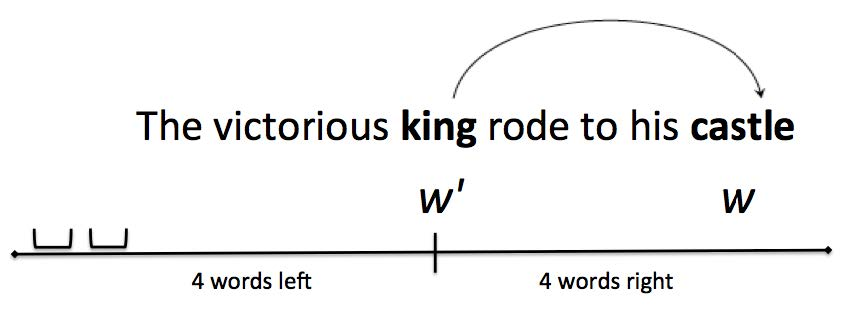
\includegraphics[width=8cm]{fig_5_1.jpg} 
	\caption{An example of the skip-gram model: we choose "king" as the active word and want to predict probabilities of words (say "castle") within a window of size 4.}\label{fig_5_1}
\end{figure}
\begin{figure}[h] 
	\centering 
	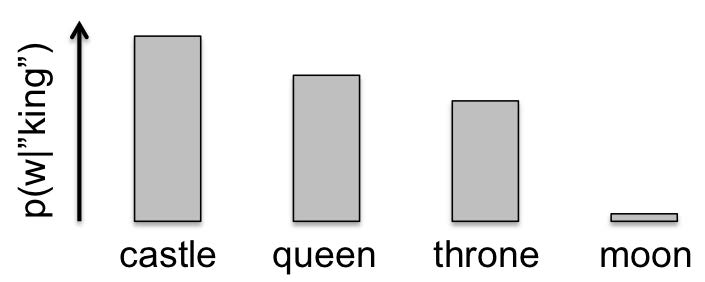
\includegraphics[width=5cm]{fig_5_2.jpg} 
	\caption{The probabilities of some words given word "king". It shows that "castle", "queen", and "throne" appear frequently near "king", and these words are therefore believed to be closely related to "king". We believe that the distribution of co-occurring words itself to some degree determines the lexical semantics}\label{fig_5_2}
\end{figure}
\par Specifically, we want to predict context words given an "active" word, which is known as the Skip-gram Model. The skip-gram model predicts the probability that $w$ occurs in context window of $w'$: $p_{\theta}(w|w')$, which captures statistic dependencies between words, as illustrated in Figure \ref{fig_5_1}. The skip-gram model, as an instance of Distributional Context Models, or Distributional Semantics Models, assumes that the distribution of co-occurring words determines lexical semantics (Figure \ref{fig_5_2}).
\section{Basic Model}
The objective function, or the predictive score, of our model is naturally chosen to be the log-likelihood. Assuming that given $w$, all words within a window are independent of each other, we obtain
\begin{equation}\label{eq_5_log_l}
\mathcal{L}(\theta;{\bf w})=\sum_{t=1}^{T}\sum_{\Delta \in \mathcal{I}}\log p_{\theta}(w^{(t+\Delta)}|w^{(t)})
\end{equation} 
where $\theta$ represents model parameters and defines the conditional probability distribution over the vocabulary given some words from the vocabulary; ${\bf w}=\{w^{(1)},\dots,w^{(T)}\}$ is the sequence of words and is implicitly padded to handle border cases; $\mathcal{I}=\{-R,\dots,-1,1,\dots,R\}$ defines a window of offsets, where we want to make prediction. Note that alternatively, we can also consider word pairs within the same sentence rather than in some windows.
\begin{remark}
	When considering word-pairs using windows, we neglect $p_{\theta}(w|w)$ for word $w$, i.e. $0\notin \mathcal{I}$, because it seems more or less meaningless to consider the word given itself. Although, it does happen that a word appears multiple times within a window, the model described above works out well in practice.
\end{remark}
\par Then we can just perform a maximum likelihood estimation to solve or optimal model parameters $\hat{\theta}$:
\begin{equation*}
\hat{\theta} = \mathop{\arg\max}_{\theta}\mathcal{L}(\theta;{\bf w})
\end{equation*}
which prefers models that assign high probability to observed context. Now the remaining question is: how should we define an appropriate model $p_{\theta}(w|w')$? 
\par Recall that we want to find a latent vector representation (embedding) of words. Specifically, our goal is to find the following mapping:
\begin{equation*}
w \mapsto ({\bf x}_w,b_w)\in \mathbb{R}^{d+1},\quad (\text{vector }+\text{ bias})
\end{equation*}
where for natural languages $d$ is usually chosen to be around $500$, and we will see the advantages to separate the bias term shortly. We hope this vector representation captures the semantics of words, as illustrated in Figure \ref{fig_5_3}. Given two vectors, the inner product is one of the simplest thing we can apply and has a nice interpretation in the sense of measuring similarities. We can therefore define a log-bilinear model by
\begin{equation}\label{eq_5_log_bi}
\log p_{\theta}(w|w')=\langle {\bf x}_w,{\bf x}_{w'}\rangle + b_w + {\rm const}
\end{equation}
where we use a symmetric bilinear form to fit the log-probabilities, but as we will see later, we can break the symmetry by introducing a different embedding $y_{w'}$ for the "active" word and use $\langle x_w,y_{w'}\rangle$ instead. Recall that in matrix factorization, we often fit the data directly with the inner products, here everything is in a log scale. The bias term gives some words more importance regardless of the conditional word and therefore to some degree handles different word frequency. The last term is a normalization constant. Then we see the log-bilinear model has the following effects:
\begin{itemize}
	\item the unspecific effect: $b_w \uparrow\ \Longrightarrow p_{\theta}(w|w')\uparrow \forall w'$,
	\item the specific effect: $\angle({\bf x}_w,{\bf x}_{w'})\downarrow\ \Longrightarrow p_{\theta}(w|w')\uparrow$.
\end{itemize}
Therefore we can say that in some sense the inner products model the interactions between words, and the biases describe the marginals of each word.
\begin{remark}
	One might ask, if we embed each word with only one vector, will this be a reasonable semantic representation for words with multiple (especially very different) meanings? For example, the word "cloud" has one meaning that is closely related to "sky", as in Figure \ref{fig_5_3}, but also has another meaning which should be closer to "computation". It turns out that in the representation learned by the model we described, the words has close meaning to "sky", as well as words has close meaning to "computation", form a small, i.e. low-dimensional, affine subspace, and the embedding for "cloud" has large inner products with both these two affine subspaces but much smaller for others. Still, multiple representation for a single word is a possible direction for word embedding, but we have to keep in mind that we have no idea what is the right thing to do.
\end{remark}
\begin{figure}[t] 
	\centering 
	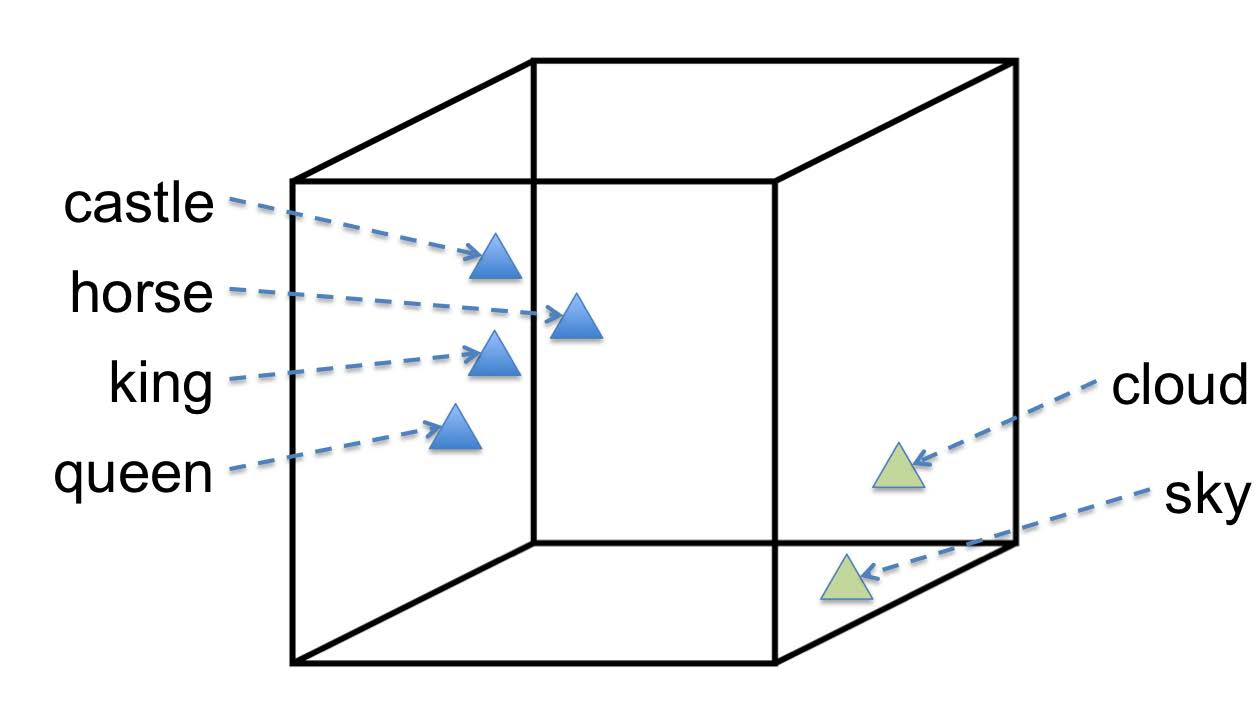
\includegraphics[width=5cm]{fig_5_3.jpg} 
	\caption{An example of words embedded to a vector space that captures semantics.}\label{fig_5_3}
\end{figure}
\par Now we can derive the normalization constant by first neglecting the constant in our log-bilinear model (\ref{eq_5_log_bi}) and exponentiating both side to give
\begin{equation*}
p_{\theta}(w|w')=\frac{\exp[\langle {\bf x}_w,{\bf x}_{w'}\rangle + b_w]}{Z_{\theta}(w')}
\end{equation*}
where
\begin{equation*}
Z_{\theta}(w')= \sum_{v\in \mathcal{V}} \exp[\langle {\bf x}_v,{\bf x}_{w'}\rangle + b_v]
\end{equation*}
is a partition function preventing naively making everything large. In the following sections, we will take a closer look into our model and discuss methods to learn the model parameters (word embeddings):
\begin{equation*}
\theta = (({\bf x}_w,b_w)_{w\in \mathcal{V}})\in \mathbb{R}^{(d+1)\cdot |\mathcal{V}|}.
\end{equation*}
Before we go to the learning algorithms of model parameters, it is worth spending sometime taking another view to understand the role of $b_w$.
\begin{remark}
	The bias term $b_w$ also plays a role to avoid ${\bf x}_w$ to be too large, which leads to separate modeling of word interactions and marginals. Since in (\ref{eq_5_log_bi}), there is no explicit regularization on the norm of ${\bf x}_w$, then if we want to evaluate the similarity by computing the inner products of word embeddings we need to be more careful. Consider a toy example in $\mathbb{R}^2$, where we have
	\begin{equation*}
	{\bf x}_1 =(1, 0),\ {\bf x}_2=(1,0.1),\ {\bf x}_2=(1,10)
	\end{equation*}
	and 
	\begin{equation*}
	\langle {\bf x}_1,{\bf x}_2\rangle = \langle {\bf x}_1,{\bf x}_3\rangle.
	\end{equation*}
	Without a bias term, a model may model different importance of words by assigning embeddings with different length. However, an embedding with larger norm will in general lead to larger inner products in magnitude, which will be problematic for the model interpretability. The introduction of $b_w$ helps relieve this problem, and in this case the $\{{\bf x}_w\}$ are usually self-normalized to 1 after training in practice. (This remark is written based on my memory of how Prof Thomas replied to a similar question of mine during the lecture and might not be correct. If you have an idea of how things should be, please send me an e-mail\footnote{yufeiyu@student.ethz.ch} and leave some comments!)
\end{remark}
\section{Skip-Gram Model}
Substituting our log-bilinear model (\ref{eq_5_log_bi}) into the log-likelihood (\ref{eq_5_log_l}) yields
\begin{align*}
\mathcal{L}(\theta;{\bf w})=\sum_{t=1}^{T}\sum_{\Delta\in \mathcal{I}}[\quad \quad \quad \quad b_{w^{(t+\Delta)}}&\quad {\rm ok} \\
+ \langle {\bf x}_{w^{(t+\Delta)}},{\bf x}_{w^{(t)}}\rangle&\quad \text{bi-linear}\longleftarrow \#1 \\
- \log \sum_{v\in \mathcal{V}} \exp[\langle {\bf x}_v,{\bf x}_{w^{(t)}}\rangle + b_v]&\quad \text{large cardinality} \longleftarrow \#2 \\
&].
\end{align*} 
There are two possible modifications to the basic model: one is on the bi-linear term, where we introduce extra distributions to make our model more flexible; the other one is on the partition function since the current version requires evaluation on a term with very large cardinality in every iteration.
\subsection{Modification \# 1: Context vectors}
As mention before, we can break the symmetry of the bi-linear model by using different embeddings for the conditional word and the words we want to predict. Specifically, we distinguish the output vocabulary $\mathcal{V}$ and the input vocabulary $\mathcal{C}$ and introduce two different embeddings:
\begin{itemize}
	\item ${\bf x}_w$: output embeddings, $w\in \mathcal{V}$
	\item ${\bf y}_w$: input embeddings, $w\in \mathcal{C}$.
\end{itemize}
Thus, we now use a mixed inner product instead:
\begin{equation*}
\log p_{\theta}(w|w')=\langle {\bf x}_w,{\bf y}_{w'}\rangle + b_w + {\rm const}.
\end{equation*}
By introducing extra parameters we increase the modeling flexibility but also the model dimensionality. We can alternatively apply a simpler model with ${\bf x}_w={\bf y}_w$ for $w\in \mathcal{V}\cap \mathcal{C}$, but it is not very commonly used.
\subsection{Modification \# 2: Objective}
The hardness of optimizing the log-likelihood objective (\ref{eq_5_log_l}) mainly comes from the partition function. A feasible fix for this problem is to alternatively optimizing other objectives whose learned parameters are also optimal for the original problem, such as
\begin{itemize}
	\item contrastive divergence (word2vec, Mikolov et al. 2013)
	\item negative sampling (Mikolov et al. 2013)
	\item pointwise mutual information (Levy \& Goldberg 2014)
	\item weighted squared loss (GloVe, Pennigton et al. 2013)
\end{itemize}
which is still a active area of research. In the following, we will discuss the negative sampling method, and we will see the objective used in GloVe in section \ref{sec_5_glove}.
\subsection{Negative Sampling}
\par The negative sampling, which is a simplified version for a more general method: \emph{noise contrastive estimation} and is used in the original skip-gram paper, reduces the estimation to binary classification tasks. The main idea is to sample positive word pairs from observed data and negative pairs from another distribution, and we train our model to distinguish there pairs. Specifically, we first introduce a contrastive, or negative, distribution $p_n(i,j)$ that is the probability to generate negative examples of word pairs $(w_i,w_j)$ and can be defined quite arbitrarily. Then with the following notations:
\begin{itemize}
	\item observed pairs (taken from some windows)$\Longrightarrow$ positive training examples $\Delta^+$
	\item pairs sampled from $p_n$ $\Longrightarrow$ negative training examples $\Delta^-$
\end{itemize}
we can perform a logistic regression, i.e. maximizing (recall that we have $\sigma(z):=\frac{1}{1+\exp(-z)}$ and $1-\sigma(z)=\sigma(-z)$)
\begin{align}
\mathcal{L}(\theta) &= \sum_{(i,j)\in \Delta^+} \log p_{\theta} ((i,j)\in\Delta^+) + \sum_{(i,j)\in \Delta^-} \log p_{\theta} ((i,j)\notin\Delta^+) \notag\\
&=\sum_{(i,j)\in \Delta^+} \log \sigma(\langle {\bf x}_i, {\bf y}_j\rangle) +\sum_{(i,j)\in \Delta^-} \log [1-\sigma(\langle {\bf x}_i, {\bf y}_j\rangle)]\notag\\
\label{eq_5_ns_lg}&=\sum_{(i,j)\in \Delta^+} \log \sigma(\langle {\bf x}_i, {\bf y}_j\rangle) +\sum_{(i,j)\in \Delta^-} \log \sigma(-\langle {\bf x}_i, {\bf y}_j\rangle)
\end{align}
where we usually still use the bias terms, but for simplicity we have absorbed the bias term into the vectors by
\begin{equation*}
{\bf x}_i\rightarrow ({\bf x}_i, b_i),\ {\bf y}_j\rightarrow ({\bf y}_j, 1).
\end{equation*}
\par For the choice of negative distribution, it is good to make it reasonably more random, i.e. to have $p_n(i,j)$ with a positive correlation to $P(w_i)P(w_j)$. In the sampling of positive pairs we still first pick an "active" word $w_j$ and sample $w_i$ from a window. It turns out to work well by first re-using the active words $w_j$, and sample "random" context words: $w_i\propto P(w_i)^\alpha$ for some positive $\alpha$, e.g. $\alpha = 3/4$, which magically works well in practice. Although people do not know why this $\alpha = 3/4$ works, it appears to have an effect to exponentially dampen frequent words.
\par Although it might seems to be reasonable to sample as many positive pairs for negative pairs, it turns out an oversampling by a factor $k$ shows better performance in practice, where usually we have $k=2-20$. For larger data sets, people usually use smaller $k$.
\subsubsection{Negative Sampling \& PMI}
Another way to understand what we are doing in negative sampling is by considering what is the best our model can do if it models everything correctly. From the Bayesian view, the best thing we can do for predicting whether a pair is a positive one is to make prediction based on the posterior distribution $p(+|(i,j))$. Applying the Bayes' theorem we obtain
\begin{equation}\label{eq_5_ns_post}
p(+|(i,j)) = \frac{p(+)p((i,j)|+)}{p(+)p((i,j)|+)+p(-)p((i,j)|-)}
\end{equation}
which yields the Bayesian optimal discriminant for $\mathcal{L}$ define in (\ref{eq_5_ns_lg})
\begin{equation*}
h^*_{ij}=\sigma^{-1}(p(+|(i,j))) = \log \frac{p(+|(i,j))}{1-p(+|(i,j))}
\end{equation*}
where we have used $\sigma^{-1}(z)=\log \frac{z}{1-z}$. The prior in (\ref{eq_5_ns_post}) is defined by the oversampling rate, i.e. $p(-)/p(+)=k$, and we have
\begin{equation*}
p((i,j)|+)=p(w_i,w_j),\ p((i,j)|-)=p_n(w_i,w_j).
\end{equation*}
Substituting these into the posterior (\ref{eq_5_ns_post}), we get
\begin{equation*}
h^*_{ij}=\log\frac{p(w_i,w_j)}{p_n(w_i,w_j)}+\log \frac{1}{k} = \log\frac{p(w_i,w_j)}{p_n(w_i,w_j)}+\log \frac{\kappa}{1-\kappa}
\end{equation*}
where $\kappa=1/(k+1)$. For $k=1$ (no oversampling) and $p_n(w_i,w_j)=p(w_i)p(w_j)$, the optimal embedding therefore satisfies
\begin{equation}\label{eq_5_ns_pmi}
\langle {\bf x}_i,{\bf y}_j \rangle \approx h^*_{ij} = \log\frac{p(w_i,w_j)}{p(w_i)p(w_j)} = {\rm PMI}(w_i,w_j)
\end{equation}
where ${\rm PMI(w_i, w_j)}$ is the \emph{pointwise mutual information} (PMI) between $w_i$ and $w_j$. If we write (\ref{eq_5_ns_pmi}) in a matrix form, we get
\begin{equation*}
{\bf X}^T{\bf Y}\approx{\rm PMI},\ {\bf X}=({\bf x}_1,\dots,{\bf x}_{|\mathcal{V}|}),\ {\bf Y}=({\bf y}_1,\dots,{\bf y}_{|\mathcal{C}|}).
\end{equation*}
We see that in this case, the negative sampling method actually performs a low-rank approximation to the pointwise mutual information matrix.
\section{GloVe}\label{sec_5_glove}
GloVe uses another strategy to deal with the normalization term. The main idea is to change the problem from maximizing the log-likelihood to a regression problem. Before we discuss the details, let us first introduce some notations. First we summarize the data in a co-occurrence matrix given by
\begin{align*}
{\bf N}=(n_{ij})&\in \mathbb{N}^{|\mathcal{V}|\cdot |\mathcal{C}|}\\
n_{ij} = \text{\# occurence of }w_{i}&\in\mathcal{V}\text{ in context of }w_j\in \mathcal{C}.
\end{align*}
Note that ${\bf N}$ is a very sparse matrix with most of its entry $0$ and can be computed in one pass over the text corpus. The concept "context" can be the window in the skip-gram model, but it is more flexible. Then, the new objective is a weighted least squares fit of the log-counts of observed data given by
\begin{equation}\label{eq_5_glv_obj}
\mathcal{H}(\theta;{\bf N})=\sum_{i,j}f(n_{ij})\left(\underbrace{\log n_{ij}}_{\text{target}}-\underbrace{\log \tilde{p}_\theta(w_i,w_j)}_{\text{model}}\right)^2
\end{equation}
with an unnormalized distribution
\begin{equation*}
\tilde{p}_{\theta}(w_i,w_j)=\exp[\langle {\bf x}_i,{\bf y}_j\rangle +b_i+c_j]
\end{equation*}
and a weighting function $f$, which deals with different frequencies of events and avoids computing logarithm for $n_{ij}=0$. Note that in the basic model, the normalization factor plays the role to avoid naively making everything large to maximize the log-likelihood, here the objective is a two-sided penalty and naturally escape from this problem. Also, we see that if our model fits the data perfectly, the normalized probability $p_{\theta}(w_i,w_j)$ is equal to the empirical distribution $\frac{\# (w_i,w_j)}{\# w_j}$.
\par The weighting function is usually chosen to take the following form
\begin{equation*}
f(n)={\rm min}\left\{1,\left(\frac{n}{n_{\rm max}}\right)^{\alpha}\right\},\ \alpha\in (0,1]\ {\rm e.g.}\ \alpha=\frac{3}{4}.
\end{equation*}
As shown in Figure \ref{fig_5_4}, this weighting function has the following motivations:
\begin{itemize}
	\item the cut-off at $n_{\rm max}$ limits the influence of large counts (frequent words);
	\item $f(n)\rightarrow 0$ for $n\rightarrow 0$: as small counts (rare events) are very noisy;
	\item the exponent $\alpha$ is usually heuristically chosen.
\end{itemize}
\begin{figure}[h] 
	\centering 
	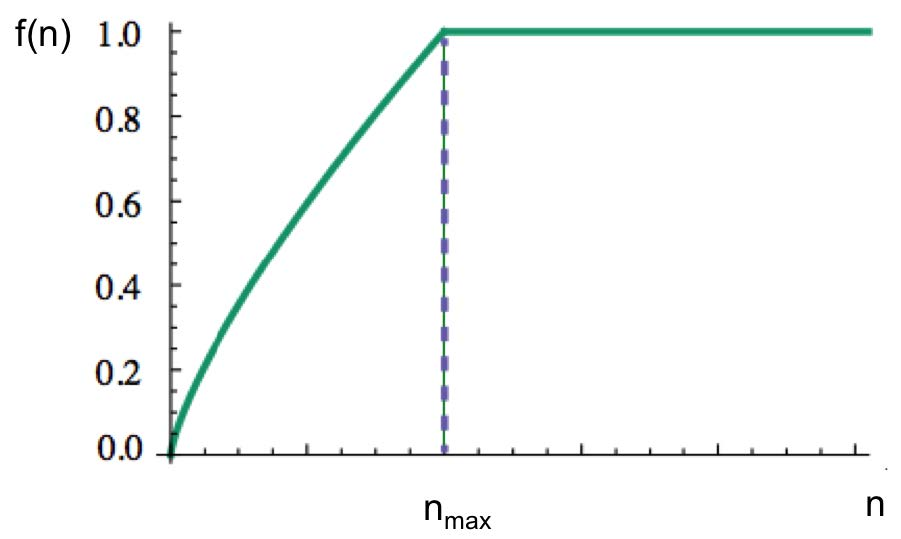
\includegraphics[width=5cm]{fig_5_4.jpg} 
	\caption{The plot of weighting function $f(n)$.}\label{fig_5_4}
\end{figure}
\subsection{Interlude: Normalized vs. Unnormalized Models}
\par At this point, it is worth comparing normalized models and unnormalized ones in a more general view. A normalized model in general over state space $\Omega$ takes the form of
\begin{equation*}
p(w)=\frac{\exp[h(w)]}{\sum_{w'\in \Omega}\exp[h(w')]}
\end{equation*}
and requires computation of the partition function. The log-likelihood is given by
\begin{equation*}
\mathcal{L}=\sum_{t}\log p(w_t)
\end{equation*}
and we have
\begin{equation*}
h(w)\uparrow\ \Longrightarrow p(w)\uparrow\ \Longrightarrow \log p(w)\uparrow\ \Longrightarrow \mathcal{L}\uparrow,
\end{equation*}
which is counterbalanced by normalization: we cannot naively make $h(w)$ large for every $w$ in order to maximize $\mathcal{L}$.
\par An unnormalized model in general, on the other hand, usually take the form of
\begin{equation*}
\tilde{p}_{\theta}(w)=\exp[h(w)]
\end{equation*}
where the exponential forces non-negativity, and no computation of partition function is required. For unnormalized models, two-sided loss functions are frequently used to make $\tilde{p}_{\theta}(w)$ neither too large nor too small. For example, GloVe uses quadratic loss with log-counts as targets.
\subsection{GloVe Optimization}
First we show that the optimization of GloVe can be regarded as a (weighted) matrix Decomposition task. Without loss of generality, we absorb bias into vectors by letting
\begin{equation*}
x_{w,d-1}=1,\ x_{w,d}=b_w\ {\rm and}\ y_{w,d-1}=c_w,\ y_{w,d}=1.
\end{equation*}
\begin{remark}\label{rmk_5_constraints}
	In the following discussion from the slides also during the lecture, after using a matrix notation, the constraint on the $(d-1)$-th dimension of ${\bf x}_w$ and the $d$-th dimension of ${\bf y}_w$ are ignored. Like in (\ref{eq_5_mf_prob}), the minimization is taken over ${\bf X,Y}$ without explicit constraints. One possible explanation is the constraints are made implicitly, but this contradicts the argument of ``go beyond SVD'' in the slide. 
\end{remark}
Then we can write everything in matrix forms by defining
\begin{align*}
&{\bf M}=(m_ij),\ m_{ij}:=\log n_{ij}\\
&{\bf X}:=[{\bf x}_{w_1}\cdots{\bf x}_{w_{|\mathcal{V}|}}],\ {\bf Y}:=[{\bf y}_{w_1}\cdots {\bf y}_{w_{|\mathcal{C}|}}].
\end{align*}
We therefore see that for GloVe with $f:=1$, optimizing the objective (\ref{eq_5_glv_obj}) is equivalent to solving a matrix factorization problem:
\begin{equation}\label{eq_5_mf_prob}
\min_{\bf X,Y}\|{\bf M}-{\bf X}^T{\bf Y}\|^2_F
\end{equation}
whose optimal solution is given by (if without the extra constraints, see remark \ref{rmk_5_constraints}) Eckart-Young Theorem (\ref{thm_1_EY}) via SVD noting that the form ${\bf X}^T{\bf Y}$ implies a rank constraint implicitly. However, for a general fixed weight for each entry, we need to go beyond SVD, and this corresponds to solve a matrix factorization problem with a weighted Frobenius norm (Definition \ref{def_3_wtd_f_norm}), and is known to be hard in general. However, for GloVe with weighting function 
\begin{equation*}
f(n_{ij}):=\begin{cases}
1 & {\rm if}\ n_{ij}>0,\\
0 & {\rm otherwise}.
\end{cases}
\end{equation*}
solves a matrix completion problem
\begin{equation*}
\min_{\bf X,Y} \sum_{i,j:n_{ij}>0} (m_{ij}-({\bf X}^T{\bf Y})_{ij})^2
\end{equation*}
which falls into a very similar setting we have discussed in section \ref{sec_3_alg_for_mc}, and all the methods like alternating least squares can be applied here.
\par For a general setting of GloVe, the non-convexity makes it hard to find the global minimal, and methods like gradient descent are often used to find a solution. Specifically, for gradient descent (aka steepest descent), we apply the following updating rules until convergence:
\begin{equation*}
\theta^{\rm new}\leftarrow \theta^{\rm old}-\eta \nabla_{\theta}\mathcal{H}(\theta;{\bf N}),\ \eta>0\ (\text{step size})
\end{equation*}
where $\mathcal{H}(\theta;{\bf N})$ is the GloVe objective function given by (\ref{eq_5_glv_obj}), and 
\begin{equation*}
\theta=(({\bf x}_w)_{w\in \mathcal{V}},({\bf y}_w)_{w\in \mathcal{C}})
\end{equation*}
are model parameters, i.e. embeddings. However, since the full gradient is often too expensive to compute for a single update, stochastic optimization is more commonly used. For stochastic gradient descent (SGD), we sample $(i,j)$ such that $n_{ij}>0$ uniformly at random, and we perform a "cheap" update for ${\bf x}_i$ and ${\bf y}_j$ with
\begin{align*}
{\bf x}^{\rm new}_i &\leftarrow {\bf x}_i + 2\eta f(n_{ij})(\log n_{ij}-\langle {\bf x}_i,{\bf y}_j \rangle){\bf y}_j\\
{\bf y}^{\rm new}_j &\leftarrow {\bf y}_j + 2\eta f(n_{ij})(\log n_{ij}-\langle {\bf x}_i,{\bf y}_j \rangle){\bf x}_i.
\end{align*}
\begin{remark}
	Again we see that there are no explicit constraints on the updates to ensure $x_{w,d-1}=1$ and $y_{w,d}=1$. A possible remedy is applying projected gradient descent instead to force the constraints.
\end{remark}
\section{Word embeddings}
The word embeddings found by distributional context models like skip-gram model turn out to capture semantics of words as expected. For example, the nearest words to "frog" in the embedding vector space are actually frogs, as illustrated in Figure \ref{fig_5_5}, which is remarkable since the model even do not know what a frog looks like.
\begin{figure}[h] 
	\centering 
	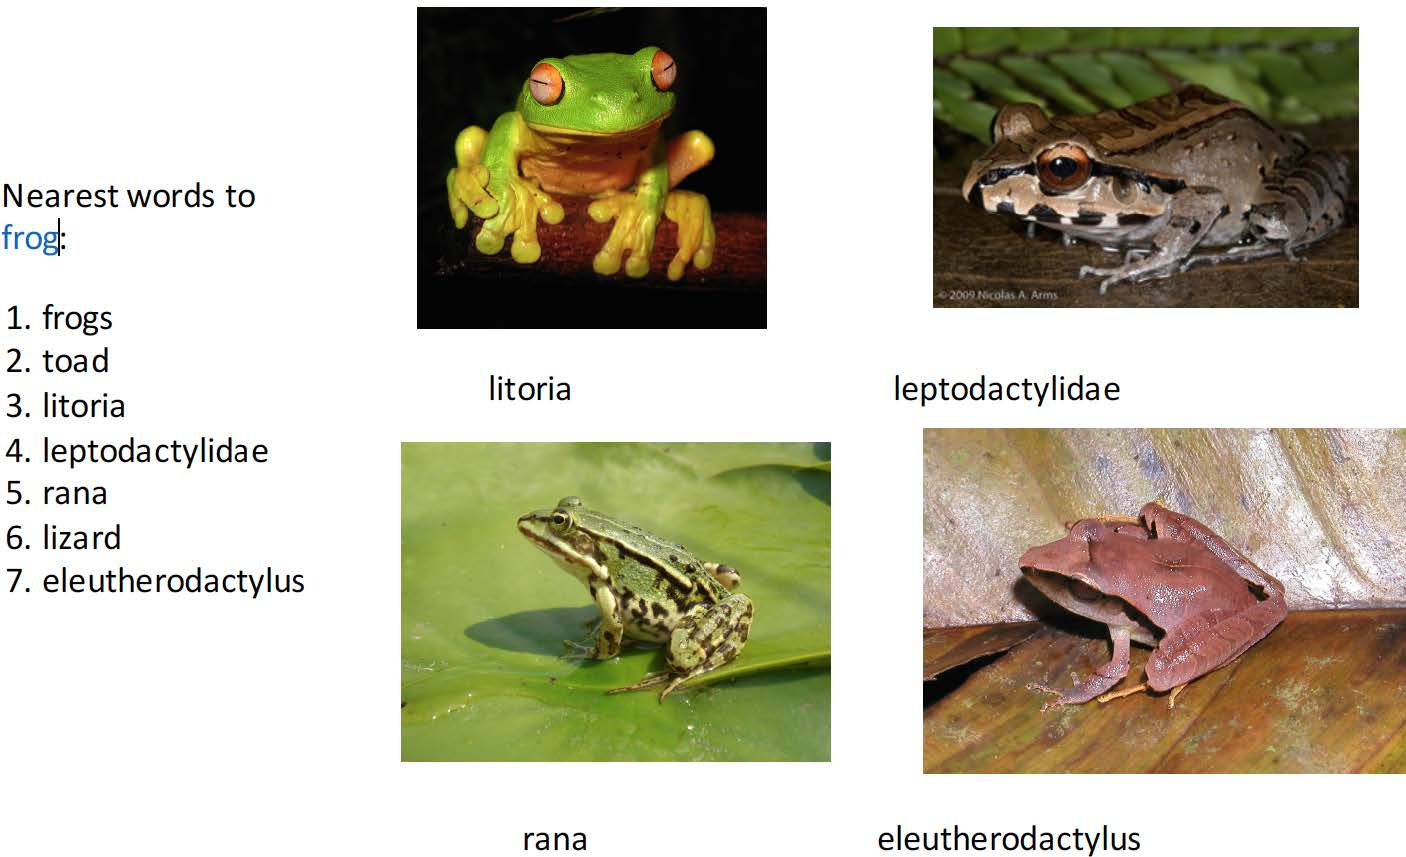
\includegraphics[width=10cm]{fig_5_5.jpg} 
	\caption{The nearest words to "frog" in embedding space.}\label{fig_5_5}
\end{figure}
\par Another interesting property of word embeddings is that it has an affine structure which captures analogies and relatedness. Think of a $a:b::c:?$ type problem, where we need to find a word $d$ that plays a similar role to $c$ as $a$ to $b$. For example, for man:woman::king:? the word "queen" will be a reasonable candidate for $d$. We see that, a model solves this type of problem captures word analogies. Mikolov et al. (2013) proposed that simple algebraic operations could be applied to embeddings to find an analogy prediction. Let ${\bf x}_a$ be the vector for $a$ and so on. For the $d$ such that the analogy holds, we expect
\begin{equation*}
{\bf x}_b - {\bf x}_a \approx {\bf x}_d-{\bf x}_c.
\end{equation*}
We can find such $d$ by searching in the vector space for the word closest to ${\bf x}_b-{\bf x}_a+{\bf x}_c$ measured by cosine distance. Specifically, we have
\begin{equation*}
d= \mathop{\arg\max}_{i\in \mathcal{V}\backslash\{a,b,c\}} \cos({\bf x}_i, {\bf x}_b-{\bf x}_a+{\bf x}_c) =\mathop{\arg\max}_{i\in \mathcal{V}\backslash\{a,b,c\}}\frac{({\bf x}_b-{\bf x}_a+{\bf x}_c)^T{\bf x}_i}{\|{\bf x}_b-{\bf x}_a+{\bf x}_c\|}
\end{equation*}
where the second equality holds for normalized word embeddings. Figure \ref{fig_5_6} shows a 2-d projected visualization for analogous word pairs found by word embeddings. We see that, the word embeddings capture the relatedness of man to woman quite well. However, the antonyms ("cheap" vs. "expensive") are usually not well captured.
\begin{figure}[h] 
	\centering 
	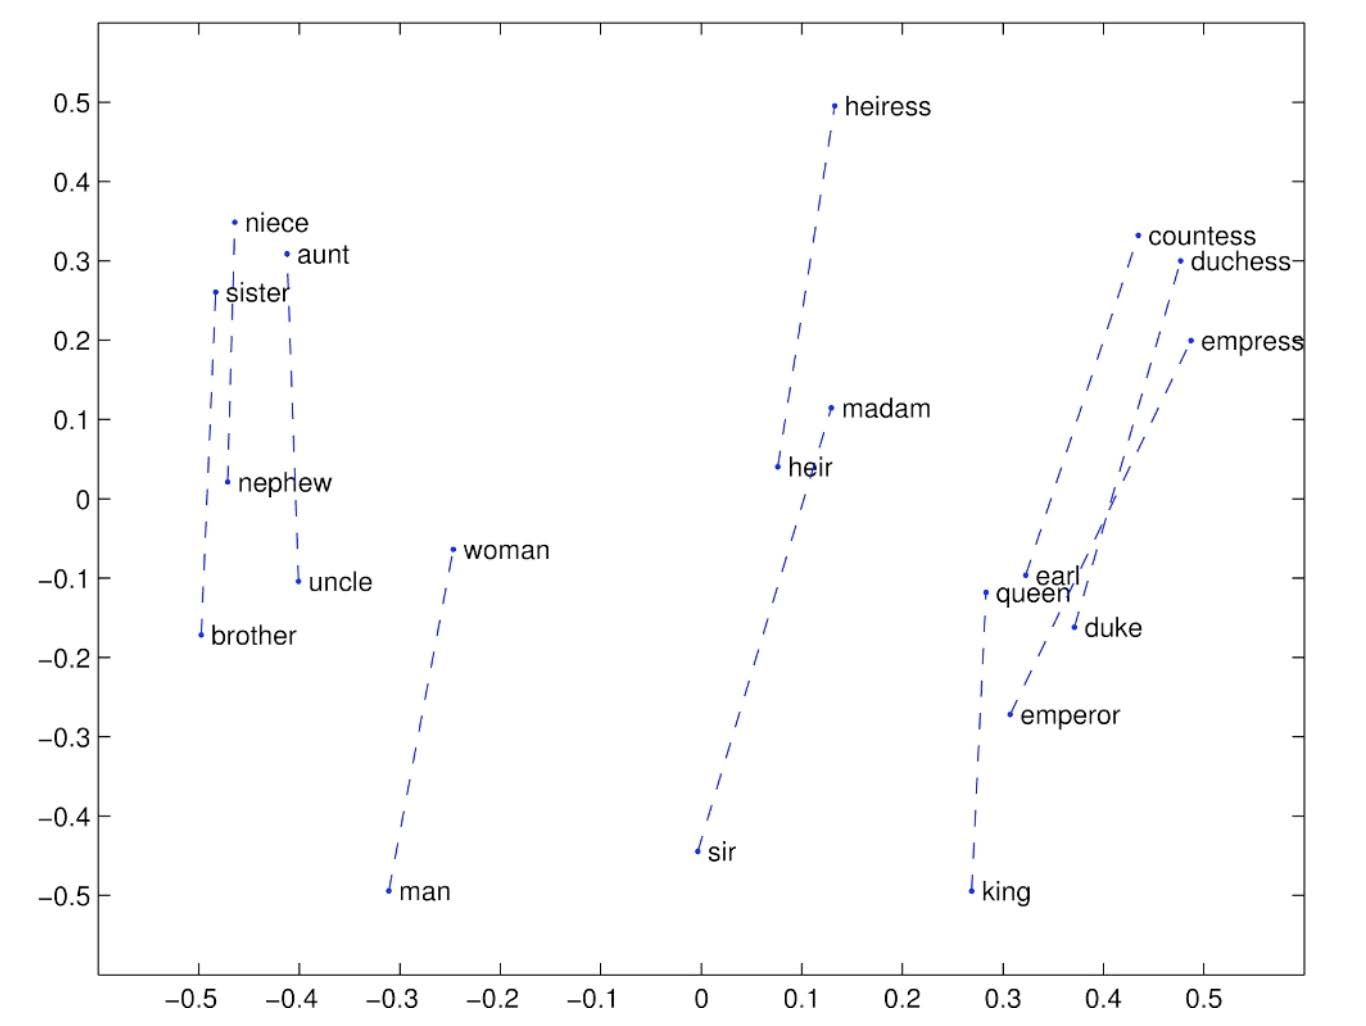
\includegraphics[width=8cm]{fig_5_6.jpg} 
	\caption{2-d projection for word vector analogies found by optimizing the cosine distance for word embeddings.}\label{fig_5_6}
\end{figure}
\par The last thing to discuss of word embeddings is the similar structures of different natural languages. The structures of human languages turn out to be quite similar up to orthogonal transformations (OT) (recall that the methods we have proposed can only find solutions that are unique up to OT since the inner products are invariant under OT). For two languages, if we have some word pairs each of which are of the same meaning, we can then use the embeddings of these pairs to do embedding alignment with orthogonal transformations after which we have words with the same meaning correspond to the same (or close) embedding. People have found that, after alignment, unobserved words with the close meanings also have similar embeddings, which is a remarkable result for machine translation. This suggests also an easy way of creating multilingual embedding space.
\par It is worth mentioning that the idea of word embeddings can also been generalized to sentence or document embeddings. It need more sophisticated analysis and methods like convolutional or recurrent neural network, but is out of the scope of this course.
\begin{figure}[h] 
	\centering 
	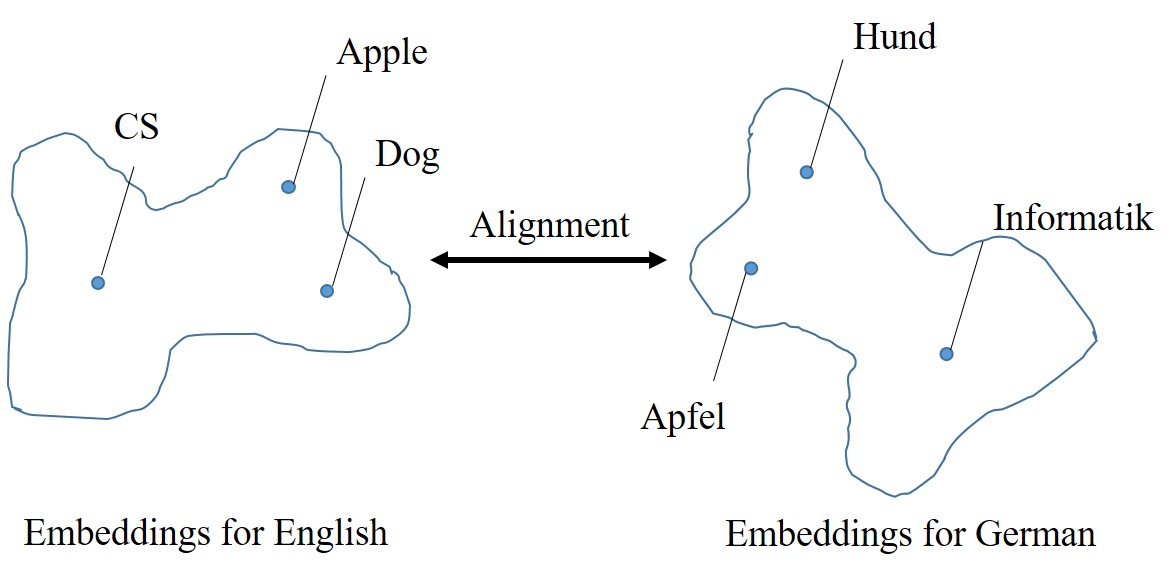
\includegraphics[width=10cm]{fig_5_7.jpg} 
	\caption{Embedding alignment for human languages}\label{fig_5_7}
\end{figure}
\end{document}